\documentclass{article}
\usepackage[utf8]{inputenc}
\usepackage[a4paper, margin=2.5cm]{geometry}
\usepackage{graphicx}
\usepackage[french]{babel}

\usepackage[default,scale=0.95]{opensans}
\usepackage[T1]{fontenc}
\usepackage{amssymb} %math
\usepackage{amsmath}
\usepackage{amsthm}
\usepackage{bbm}
\usepackage{systeme}

\usepackage{hyperref}
\hypersetup{
	colorlinks=true,
	linkcolor=blue,
	filecolor=magenta,      
	urlcolor=cyan,
	pdftitle={Overleaf Example},
}
\urlstyle{same} %\href{url}{Text}

\theoremstyle{plain}% default
\newtheorem{thm}{Théorème}[section]
\newtheorem{lem}[thm]{Lemme}
\newtheorem{prop}[thm]{Proposition}
\newtheorem*{cor}{Corollaire}
%\newtheorem*{KL}{Klein’s Lemma}

\theoremstyle{definition}
\newtheorem{defn}{Définition}[section]
\newtheorem{exmp}{Exemple}[section]
% \newtheorem{xca}[exmp]{Exercise}

\theoremstyle{remark}
\newtheorem*{rem}{Remarque}
\newtheorem*{note}{Note}
%\newtheorem{case}{Case}



\title{Simulation : Chapitre 3 : Simulation de lois particulières}
\author{Charles Vin}
\date{2021}

\begin{document}
\maketitle

\section{Simulations de lois discrète}
On veut simuler une v.a. $ X $ à valeur dans $ \{x_1, x_2, ..., x_d\} $. \\
On connait son tableau de loi, i.e. la liste des $ P(X=x_k) $ pour chaque $ k $\\
On note $ s_k = \sum_{i=1}^{k}P(X=x_i) $. Les $ s_k $ sont les valeurs prises par la fonction de répartition de $ X $ si les $ x_i $ sont classés par ordre croissant (ce qui n'est pas forcément une bonne chose). (exemple Figure \ref{fig1})

\begin{figure}[!htbp]
	\centering
	\includegraphics*[width=.5\textwidth]{./figures3/fig1.jpg}
	\label{fig1}
\end{figure}

On tire $ U \sim unif(]0;1[) $ : on obtient $ U(w) $. On détermine l'unique $ k $ tel que $ s_{k-1} < U(w) \leq s_k $ et on pose $ Y(w) = x_k $. \\
On a alors 
\begin{align*}
	P(Y=x_k) &= P(s_{k-1} < U \leq s_k) \\
			&= s_k - s _{k-1} = P(X=x_k) 
\end{align*}
Donc $ Y $ a même loi que $ X $ \\

\textbf{Efficacité} : \\
On test successivement si $ U \leq s_1 $, si $ U \leq 
s_2 $ donc l'algorithme se termine plus vite si on classe les $ x_k $ par ordre de probabilités décroissantes : 
\[
	P(X=x_1) \geq P(X=x_2) \geq \dots \geq P(X=x_d)
.\]

\begin{exmp}[]
	On lance un palet sur la Table \ref{fig2}. $ X $ indique le nombre de points obtenus par un lancer au hasard. $ X(\Omega ) = \{0,5,10\} $. La loi de $ X $ dans la Table \ref{fig3}.
	
	\begin{table}[!ht]
		\centering
		\label{fig2}
		\begin{tabular}{|l|l|l|}
		\hline
			5 & 5 & 5 \\ \hline
			5 & 0 & 5 \\ \hline
			0 & 10 & 0 \\ \hline
			5 & 0 & 5 \\ \hline
			5 & 5 & 5 \\ \hline
		\end{tabular}
	\end{table}

	\begin{table}[!ht]
		\centering
		\label{fig3}
		\begin{tabular}{|l|l|l|l|}
		\hline
			$x\_k$ & 0 & 5 & 10 \\ \hline
			$ P(X=x\_k)$ & 4/15 & 10/15 & 1/15 \\ \hline
		\end{tabular}
	\end{table}

	On tire $ U \sim Unif(]0;1[) $\\
	Si $ U < \frac{10}{15} $  alors $ Y=5 $ sinon si $ U < \frac{14}{15} $ alors $ Y=0 $ sinon $ Y=10 $ (voir Figure \ref{fig4})

	\begin{figure}[!htbp]
		\centering
		\includegraphics*[width=.5\textwidth]{./figures3/fig4.png}
		\caption{Exemple}
		\label{fig4}
	\end{figure}

\end{exmp}

\section{Technique spécifiques pour des lois discrètes particulière}
\subsection{Loi de Bernouilli}

Si $ U \sim Unif(]0;1[), \mathbbm{1}_{U \leq p} \sim Ber(p) $ 
(voir Figure \ref{fig5})
\begin{figure}[!htbp]
	\centering
	% demander à ID
	% \includegraphics*[width=.5\textwidth]{./figures3/fig3.?}
	\caption{Technique par fonction quantiles j'ai pas l'image sorry}
	\label{fig5}
\end{figure}

\subsection{Loi binomiales et multinomiales}
Si $ U_1, U_2, ..., U_n $ sont i.i.d. de loi $ Unif(]0;1[) $ alors $ \sum_{i=1}^{n}\mathbbm{1}_{U_i \leq p} \sim Bin(n,p) $ 

\begin{note}[]
	\textbf{Rappel : } La loi multinomiales de paramètres $ (n,p_1, p_2, ..., p_k) $ où les $ p_i $ sont positifs et de somme $ 1 $ est la loi du vecteur aléatoire $ (X_1,X_2, ..., X_k) $ représentant le nombre de résultats de type obtenus en $ n $ expérience indépendantes ayant toutes une probabilité $ p_1 $ de donner le résultat de type $ 1 $, une probabilité $ p_2 $ de donner le résultat de type $ 2 $, etc.
	
	$ (X, n-X) \sim Multinomiales(n,p,1-p) \text{ si } X \sim Bim(n,p) $ 
\end{note}

La même technique permet de simuler les lois multinomiales \\ 
Si $ U_1, \dots, U_n $ i.i.d. $ Unif(]0;1[) $ 
\[
	(\sum_{i=1}^{n}\mathbbm{1}_{U \leq p_1}, \sum_{i=1}^{n}\mathbbm{1}_{p_1 < U \leq p_1 + p_2}, \sum_{i=1}^{n}\mathbbm{1}_{p_1 + p_2 < U \leq p_1 + p_2 + p_3}, \dots, \sum_{i=1}^{n}\mathbbm{1}_{p_1 + \dots + p _{k-1} < U \leq 1}) \sim Mult(n,p_1, \dots, p_k)
.\]

\subsection{Loi géométrique}

\textbf{Rappel:} La loi $ Géom(p) $ est la loi du nombre de tentatives indépendantes nécessaire pour obtenir le premier succès si chaque tentative a une proba $ p $ de succès \\

Si on simule la loi géométrique de paramètre $ p $ par cette méthode, le nombre moyen de v.a. Uniforme sur $ O $ et $ 1 $ nécessaire pour obtenir un tirage de $ X \sim Geom(p) $ est $ E(X) = \frac{1}{p} $ qui est très grand si $ p $  est très petit. Il est préférable surtout pour $ p $ petit, d'utiliser une méthode qui ne nécessite pas d'un tirage de loi uniforme.

\begin{prop}[]
	Si $ V \sim Exp(a) $ alors $ \lceil V \rceil \sim Geom(1-e^{-a})$ où $ \lceil \rceil $ est la partie entière supérieure : $ \lceil x \rceil = \min \{k \in \mathbb{Z}, x \leq k\}$ 
\end{prop}
\begin{proof}[Preuve: ]
	\begin{align*}
		P(\lceil V \rceil = k) = P(k-1 < V \leq k) &= \int_{k-1}^{k}ae^{-ax}dx \\
		&= [-e^{-ax}]_{k-1}^k \\
		&= -e^{-ak} + e^{-a(k-1)} \\
		&= e^{-a(k-1)} (1-e^{-a}) \\
		&= p(1-p)^{k-1}
	\end{align*}
	donc $ \lceil V \rceil \sim Geom(1-e^{-a}) $. Suite :
	\[
		1-e^{-a} = p \Leftrightarrow e^{-a} = 1-p \Leftrightarrow a = -\ln (1-p)
	.\]
	On sait simuler $ Exp(-\ln (1-p)) $ par $ \frac{-\ln U}{-\ln (1-p)} = \frac{\ln U}{\ln (1-p)} $ où $ U \sim Unif(]0;1[) $ \\
	CCL : Simulation de Géom(p) : 
	\[
		\lceil \frac{\ln U}{\ln (1-p)} \rceil \sim Geom(p) \text{ si } U \sim Unif(]0;1[)
	.\]
\end{proof}

\subsection{Loi de Poisson}

\begin{prop}[]
	Le nombre maximal de v.a. exponentielles indépendantes de paramètre $ a $ qu'on peut additionner sans dépasser $ 1 $ suit la loi de Poisson de paramètre $ a $. \\
	Si $ X_1, X_2, \dots $ sont i.i.d. $ Exp(a) $ 
	\[
		\forall n \in \mathbb{N}, P(\sum_{i=1}^{n}X_i \leq 1 < \sum_{i=1}^{n+1}X_i) = e^{-a}\frac{a^n}{n!}
	.\]
\end{prop}
\textbf{Conséquence:} Si $ U_1, U_2, \dots $ i.i.d $ Unif(]0;1[) $ alors l'entier aléatoire $ N $ tel que $ \prod_{i=1}^{N}U_i \geq e^{-a} > \prod_{i=1}^{N+1}U_i $ suit la loi $ Pois(a) $ \\

\textbf{Pourquoi ?} \\
\begin{align*}
	P(\sum_{i=1}^{n}X_i \leq 1 < \sum_{i=1}^{n+1}X_i) & \\
	&= \int_{\mathbb{R}^{n+1}}^{} \mathbbm{1}_{\sum_{i=1}^{n}X_i \leq 1 < \sum_{i=1}^{n+1}X_i)} \prod_{i=1}^{n+1}(ae^{-ax_i} \mathbbm{1}_{x_i > 0}) dx_1 \dots dx_{n+1} \\ 
	&= a^{n+1} \int_{\mathbb{R}^{n+1}} \mathbbm{1}_{x_1 + \dots + x_n \leq 1, x_1 + \dots + x_n + x _{n+1} 
	> 1, x_1 >0 \dots x_{n+1} > 0 } * e^{-a (x_1+ \dots + x_{n+1})} dx_1 \dots dx_{n+1} \\ 
\end{align*}
Changement de variable : 
\begin{align*}
	u_1 = x_1 						&\Leftrightarrow x_1 = u_1\\
	u_2 = x_1 + x_2 				&\Leftrightarrow x_2 = u_2 - u_1\\
	u_3 = x_1 + x_2 + x_3 			&\Leftrightarrow x_3 = u_3 - u_2\\
	\dots 							&\\
	1 + \dots + x_n 				&\Leftrightarrow x_n = u_n - u_{n-1}\\
	u_{n+1} = x_1 + \dots x_{n+1}	&\Leftrightarrow x_{n+1} = u_{n+1} - u_n\\
\end{align*}

\[
	dx_1 \dots dx_{n+1} = \left| \det \begin{pmatrix}
		\frac{\partial x_1}{\partial u_1} & \dots & \frac{\partial x_1}{\partial u_{n+1}} \\
		\frac{\partial x_2}{\partial u_1} & \dots & \frac{\partial x_2}{\partial u_{n+1}} \\
		\vdots & \dots & \vdots  \\
		\frac{\partial x_{n+1}}{\partial u_1} & \dots & \frac{\partial x_{n+1}}{\partial u_{n+1}} 
	\end{pmatrix}
	\right|  = \begin{pmatrix}
	1      & 0      & \dots  & 0          \\
	-1     & 1      & \ddots & \vdots     \\
	0      & \ddots & \ddots & 0          \\
	\vdots & \ddots & \ddots & 1         \\
	0      & \dots  & 0      & -1  & 1  
\end{pmatrix}
.\]

\underline{Nouveau cours du 23/11} \\
C'est le chaos cette matrice, j'arrive pas à la faire en latex
\begin{figure}[htbp]
	\centering
	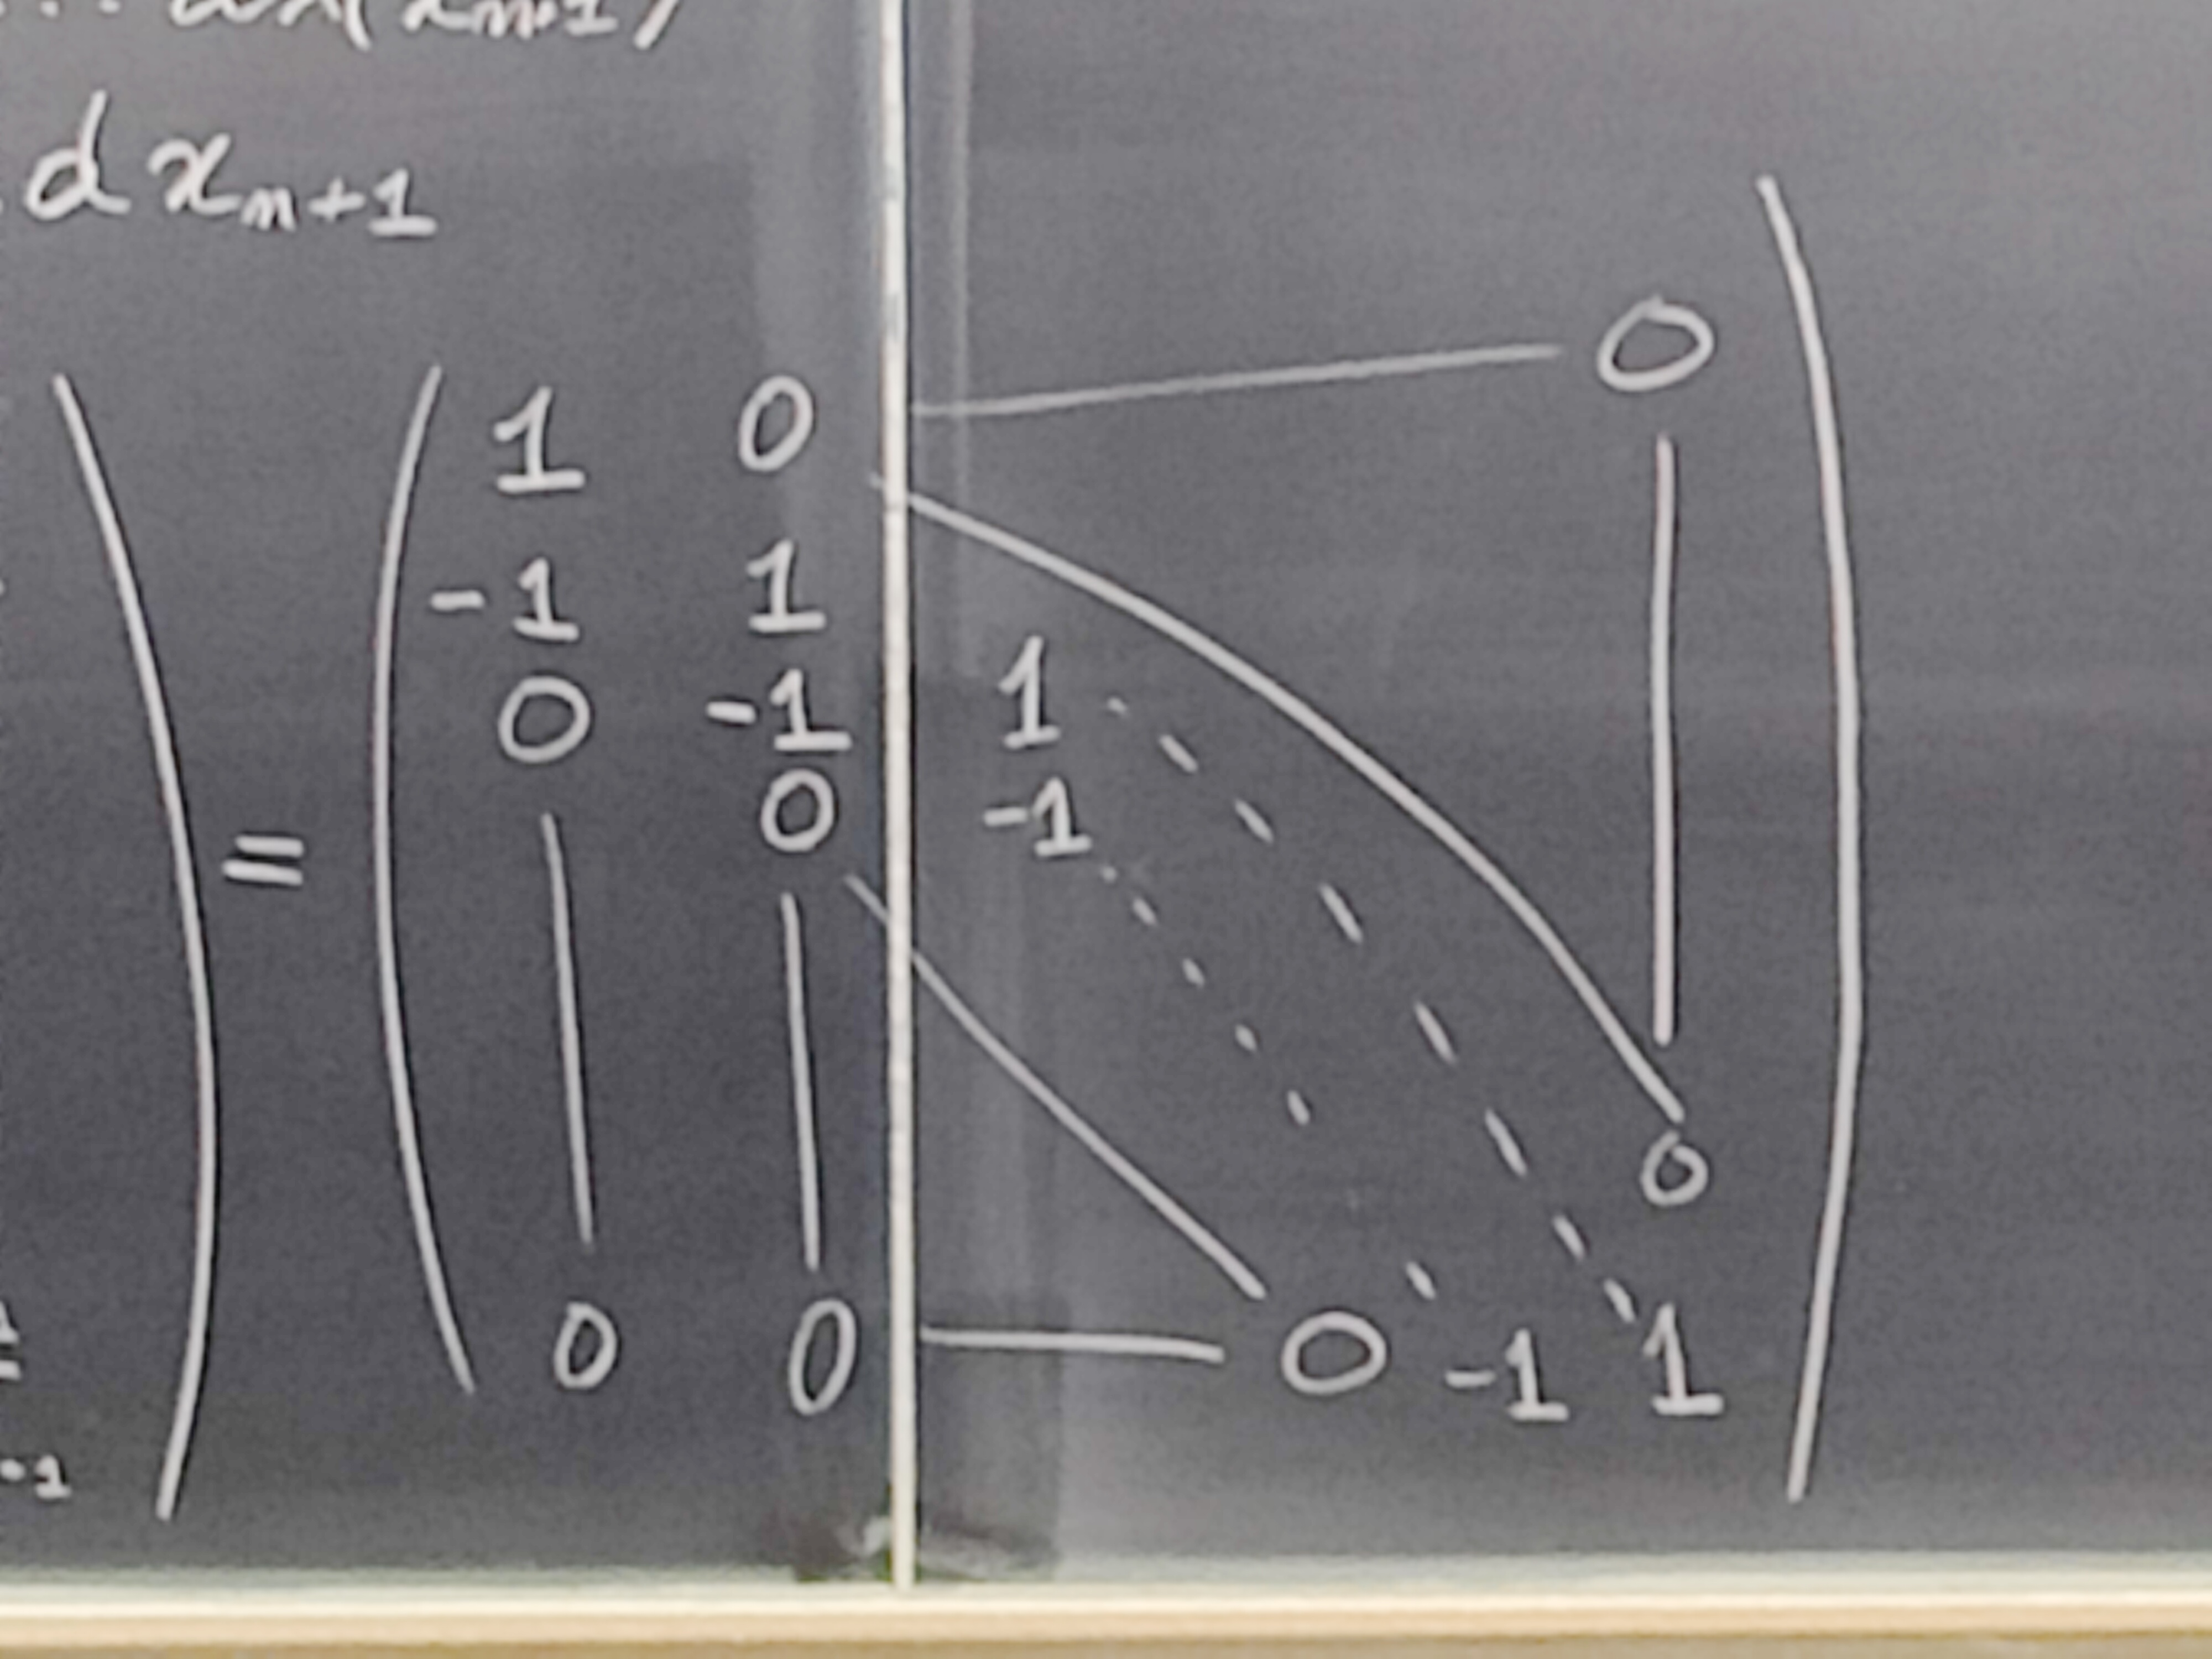
\includegraphics[width=.70\textwidth]{figures3/fig5.jpg}
	\caption{<caption>}
	\label{<label>}
\end{figure}

\[
	= \left| \det Jac(u) \right| du_1 \dots du_{n+1} = \left| 1 \right| du_1 \dots du_{n+1}
.\]

\begin{align*}
	P(\sum_{i=1}^{n}X_i \leq 1 < \sum_{i=1}^{n+1}X_i) &= a^{n+1} \int_{\mathbb{R}^{n+1}} \mathbbm{1}_{u_n \leq 1} \mathbbm{1}_{u_{n+1} > 1} e^{-a u_{n+1}} \mathbbm{1}_{u_{n+1} > u_n > \dots > u_1 > 0} \left| 1 \right| du_1 \dots du_{n+1} \\
	&= a^{n+1} \int_{\mathbb{R}^n} ( \int_{\mathbb{R}} \mathbbm{1}_{u_n < 1} \mathbbm{1}_{u_{n+1} > 1} e^{-a u_{n+1}} \mathbbm{1}_{u_{n+1} > u_n} \mathbbm{1}_{u_n > u_{n-1} > \dots > u_1 > 0}() du_{n+1}) du_1 \dots du_n \\
	&= a^{n+1} \int_{\mathbb{R}^n} \mathbbm{1}_{u_n < 1} \mathbbm{1}_{u_n > u_{n-1} > \dots > u_1 > 0} ( \int_{\mathbb{R}} \mathbbm{1}_{u_{n+1} > 1} e^{-au_{n+1}} du_{n+1}) du_1 \dots du_n \\
	&= \frac{a^{n+1}}{a}e^{-a} \int_{\mathbb{R}^n} \mathbbm{1}_{1 \geq u_n \geq u_{n-1} > \dots > u_1 > 0} du_1 \dots du_n \\
	&= a^n e^{-a} \int_{\mathbb{R}^n} \mathbbm{1}_{u_1 < u_2 < \dots <u_n} (\prod_{i=1}^{n} \mathbbm{1}_{0<u_i<1}) du_1 \dots du_n \\
	&= a^n e^{-a} P(U_1 < U_2 < \dots < U_n) \\
	&= a^n e^{-a} P(U_1 < \dots < U_n) \text{ pour } U_1, \dots, U_n \text{ i.i.d. } Unif(]0;1])
	&= a^n e^{-a} \frac{1}{n!} \text{ car tous les ordres des Ui sont équiprobables ici }
\end{align*}

CCL : Si les $ X_i $ sont i.i.d. $ Exp(a) $ alors le nombre aléatoire $ N $ de $ X_i $ tel que $ \sum_{i=1}^{N}X_i \leq 1 < \sum_{i=1}^{N+1}X_i $ satifait $ P(N=n) = \frac{a^n}{n!}e^{-a} \Leftrightarrow N \sim Pois(a)$ 

On sait que si $ U_1, \dots, U_n $ i.i.d. $ Unif(]0;1[) $ alors 
\[
	X_1 \frac{-\ln U_1}{a}, X_2 \frac{-\ln U_2}{a} \text{ i.i.d. } Exp(a)
.\]
$ N \sim Pois(a) $ si $ N $ est déterminé par
\begin{align*}
	& \sum_{i=1}^{N} \frac{-\ln U_i}{a} \leq 1 < \sum_{i=1}^{N+1} \frac{-\ln U_i}{a} \\
	& -\frac{1}{a}\ln (\prod_{i=1}^{N}U_i) \leq 1 < - \frac{1}{a}\ln (\prod_{i=1}^{N+1}U_i) \\
	& \prod_{i=1}^{N}U_i \geq e^{-a} > \prod_{i=1}^{N+1}U_i
\end{align*}

\subsection{Simulation de gaussiennes}
\textbf{Rappel: } Si $ X $ simule la $ \mathcal{N}(0,1) $ alors $ \sigma X + m $ simule $ \mathcal{N}(m, \sigma ^2) $ 

Inversion de la fonction de répartition : La fonction quantile de la $ \mathcal{N}(0,1) $ est 
\[
	\alpha \mapsto \inf \{t \in \mathbb{R}, \int_{_\infty }^{t} \frac{1}{\sqrt[]{2 \pi }} e^{- \frac{x^2}{2}} dx \geq \alpha \}
.\]
La méthode de simulation par inversion de la fonction de répartition n'est pas pratique ici

Méthode du rejet : Algorithme de Ziggurat, on l'utilisait sur les anciens processeurs, pas pratique 

Méthode de Box-Muller : Si $ U $ et $ V $ sont indépendantes de loi $ Unif(]0;1[) $ alors
\begin{align*}
	& X=\sqrt[]{-2 \ln U} \cos(2 \pi V) \\
	& Y=\sqrt[]{-2 \ln U} \sin (2 \pi V)
\end{align*}
sont indépendantes de loi $ \mathcal{N}(0,1) $ 

\begin{proof}[Preuve: ]
	Calcul de la fonction de répartion de $ X, Y $.

	Vérifions que $ \forall s,t \in \mathbb{R} $ 
	\[
		P(X \leq s, Y \leq t) = \int_{_\infty }^{s} \frac{1}{\sqrt[]{2 \pi }} e^{- \frac{x^2}{2}} dx * \int_{_\infty }^{t} \frac{1}{\sqrt[]{2 \pi }} e^{- \frac{x^2}{2}} dx
	.\]
	\begin{align*}
		P(X \leq s, Y \leq t) &= P(\sqrt[]{-2 \ln U} \cos (2 \pi V) \leq s \text{ et  } \sqrt[]{-2 \ln U} \sin (2 \pi V) \leq t) \\
		&= \int_{\mathbb{R}^2} \mathbbm{1}_{\sqrt[]{-2 \ln U} \cos (2 \pi V) \leq s} \mathbbm{1}_{\sqrt[]{-2 \ln U} \sin (2 \pi V) \leq t} \mathbbm{1}_{0 < u < 1} \mathbbm{1}_{0 < v < 1} du dv
	\end{align*}
	\begin{note}[]
		$ \mathbbm{1}_{0 < u < 1} \mathbbm{1}_{0 < v < 1} $ est le produit des densités de $ U $ et $ V $.
	\end{note}
	Changement de variable : 
	\begin{align*}
		&x=\sqrt[]{-2 \ln u} \cos(2 \pi v), u= e^{-\frac{x^2 + y^2}{2}}\\
		&y=\sqrt[]{-2 \ln u} \sin (2 \pi v), v= \\
		&x^2 + y^2 = -2 \ln u \Leftrightarrow - \frac{x^2 + y^2}{2} = \ln u \\
		&\frac{y}{x} = \tan (2 \pi v)
	\end{align*}
	
	\begin{align*}
		&]0;1[^2 \to \mathbb{R}^2 \setminus (]0;+\infty[ \times \{0\})
		&(u,v) \mapsto (x,y)
	\end{align*}
	La jacobienne : 
	\begin{align*}
		dxdy &= \left| \det \begin{pmatrix}
			\frac{\partial x}{\partial u} & \frac{\partial x}{\partial v} \\
			\frac{\partial y}{\partial u} & \frac{\partial y}{\partial v} 
		\end{pmatrix}
		\right| du dv \\
		Jac(u,v) &= \begin{pmatrix}
			\cos (2 \pi v) ( \frac{-2 * \frac{1}{u}}{2 \sqrt[]{-2 \ln u}}) & -2 \pi \sin (2 \pi v) \sqrt[]{-2 \ln u}\\
			\sin (2 \pi v) ( \frac{-2 * \frac{1}{u}}{2 \sqrt[]{-2 \ln u}}) & 2 \pi \cos (2 \pi v) \sqrt[]{-2 \ln u}\\
		\end{pmatrix} \\
		\det Jac(u,v) &= \frac{-1}{u \sqrt[]{-2 \ln u}} * 2 \pi \sqrt[]{-2 \ln u} \det \begin{pmatrix}
			\cos (2 \pi v) & -\sin (2 \pi v) \\
			\sin (2 \pi v) & \cos (2 \pi v)
		\end{pmatrix} \\
		&= \frac{-2 \pi }{u} * 1 \\ 
		dxdy &= \frac{2 \pi }{u} dudv \\
		dudv &= \frac{1}{2 \pi} e^{- \frac{x^2 + y^2}{2}}
	\end{align*}
	\begin{align*}
		P(X \leq s, Y \leq t) &= \int_{\mathbb{R}^2 \setminus (]0;+\infty[ \times \{0\} ) } \mathbbm{1}_{x \leq s} \mathbbm{1}_{y \leq t} \frac{1}{2 \pi } e^{- \frac{x^2}{2}} e^{-\frac{y^2}{2}}dxdy \\
		&= \int_{\mathbb{R}} \int_{\mathbb{R}} \mathbbm{1}_{x \leq s} \mathbbm{1}_{y \leq t} \frac{1}{2 \pi } e^{- \frac{x^2}{2}} e^{-\frac{y^2}{2}}dxdy \\
		&= \int_{\mathbb{R}} \mathbbm{1}_{y \leq t} \frac{e^{-\frac{y^2}{2}}}{\sqrt{2 \pi }} (\int_{\mathbb{R}} \mathbbm{1}_{x \leq s} \frac{e^{- \frac{x^2}{2}}}{\sqrt[]{2 \pi }} dx ) dy \\
		&= \phi (s) \phi (t)
	\end{align*}
\end{proof}







\end{document}